\documentclass[twoside]{book}

% Packages required by doxygen
\usepackage{calc}
\usepackage{doxygen}
\usepackage{graphicx}
\usepackage[utf8]{inputenc}
\usepackage{makeidx}
\usepackage{multicol}
\usepackage{multirow}
\usepackage{textcomp}
\usepackage[table]{xcolor}

% Font selection
\usepackage[T1]{fontenc}
\usepackage{mathptmx}
\usepackage[scaled=.90]{helvet}
\usepackage{courier}
\usepackage{amssymb}
\usepackage{sectsty}
\renewcommand{\familydefault}{\sfdefault}
\allsectionsfont{%
  \fontseries{bc}\selectfont%
  \color{darkgray}%
}
\renewcommand{\DoxyLabelFont}{%
  \fontseries{bc}\selectfont%
  \color{darkgray}%
}

% Page & text layout
\usepackage{geometry}
\geometry{%
  a4paper,%
  top=2.5cm,%
  bottom=2.5cm,%
  left=2.5cm,%
  right=2.5cm%
}
\tolerance=750
\hfuzz=15pt
\hbadness=750
\setlength{\emergencystretch}{15pt}
\setlength{\parindent}{0cm}
\setlength{\parskip}{0.2cm}
\makeatletter
\renewcommand{\paragraph}{%
  \@startsection{paragraph}{4}{0ex}{-1.0ex}{1.0ex}{%
    \normalfont\normalsize\bfseries\SS@parafont%
  }%
}
\renewcommand{\subparagraph}{%
  \@startsection{subparagraph}{5}{0ex}{-1.0ex}{1.0ex}{%
    \normalfont\normalsize\bfseries\SS@subparafont%
  }%
}
\makeatother

% Headers & footers
\usepackage{fancyhdr}
\pagestyle{fancyplain}
\fancyhead[LE]{\fancyplain{}{\bfseries\thepage}}
\fancyhead[CE]{\fancyplain{}{}}
\fancyhead[RE]{\fancyplain{}{\bfseries\leftmark}}
\fancyhead[LO]{\fancyplain{}{\bfseries\rightmark}}
\fancyhead[CO]{\fancyplain{}{}}
\fancyhead[RO]{\fancyplain{}{\bfseries\thepage}}
\fancyfoot[LE]{\fancyplain{}{}}
\fancyfoot[CE]{\fancyplain{}{}}
\fancyfoot[RE]{\fancyplain{}{\bfseries\scriptsize Generated on Thu Dec 26 2013 12\-:10\-:13 for S\-D\-Lpp by Doxygen }}
\fancyfoot[LO]{\fancyplain{}{\bfseries\scriptsize Generated on Thu Dec 26 2013 12\-:10\-:13 for S\-D\-Lpp by Doxygen }}
\fancyfoot[CO]{\fancyplain{}{}}
\fancyfoot[RO]{\fancyplain{}{}}
\renewcommand{\footrulewidth}{0.4pt}
\renewcommand{\chaptermark}[1]{%
  \markboth{#1}{}%
}
\renewcommand{\sectionmark}[1]{%
  \markright{\thesection\ #1}%
}

% Indices & bibliography
\usepackage{natbib}
\usepackage[titles]{tocloft}
\setcounter{tocdepth}{3}
\setcounter{secnumdepth}{5}
\makeindex

% Hyperlinks (required, but should be loaded last)
\usepackage{ifpdf}
\ifpdf
  \usepackage[pdftex,pagebackref=true]{hyperref}
\else
  \usepackage[ps2pdf,pagebackref=true]{hyperref}
\fi
\hypersetup{%
  colorlinks=true,%
  linkcolor=blue,%
  citecolor=blue,%
  unicode%
}

% Custom commands
\newcommand{\clearemptydoublepage}{%
  \newpage{\pagestyle{empty}\cleardoublepage}%
}


%===== C O N T E N T S =====

\begin{document}

% Titlepage & ToC
\hypersetup{pageanchor=false}
\pagenumbering{roman}
\begin{titlepage}
\vspace*{7cm}
\begin{center}%
{\Large S\-D\-Lpp }\\
\vspace*{1cm}
{\large Generated by Doxygen 1.8.6}\\
\vspace*{0.5cm}
{\small Thu Dec 26 2013 12:10:13}\\
\end{center}
\end{titlepage}
\clearemptydoublepage
\tableofcontents
\clearemptydoublepage
\pagenumbering{arabic}
\hypersetup{pageanchor=true}

%--- Begin generated contents ---
\chapter{Hierarchical Index}
\section{Class Hierarchy}
This inheritance list is sorted roughly, but not completely, alphabetically\-:\begin{DoxyCompactList}
\item \contentsline{section}{sdl\-:\-:Clock}{\pageref{classsdl_1_1Clock}}{}
\item \contentsline{section}{sdl\-:\-:Color}{\pageref{classsdl_1_1Color}}{}
\item \contentsline{section}{sdl\-:\-:Duration}{\pageref{classsdl_1_1Duration}}{}
\item \contentsline{section}{sdl\-:\-:Font}{\pageref{classsdl_1_1Font}}{}
\item \contentsline{section}{sdl\-:\-:Renderer}{\pageref{classsdl_1_1Renderer}}{}
\item \contentsline{section}{sdl\-:\-:Sprite}{\pageref{classsdl_1_1Sprite}}{}
\item \contentsline{section}{sdl\-:\-:Surface}{\pageref{classsdl_1_1Surface}}{}
\item \contentsline{section}{sdl\-:\-:Text}{\pageref{classsdl_1_1Text}}{}
\item \contentsline{section}{sdl\-:\-:Texture}{\pageref{classsdl_1_1Texture}}{}
\item \contentsline{section}{sdl\-:\-:Vector2$<$ T $>$}{\pageref{classsdl_1_1Vector2}}{}
\item \contentsline{section}{sdl\-:\-:Vector2$<$ float $>$}{\pageref{classsdl_1_1Vector2}}{}
\begin{DoxyCompactList}
\item \contentsline{section}{sdl\-:\-:Vector2f}{\pageref{classsdl_1_1Vector2f}}{}
\end{DoxyCompactList}
\item \contentsline{section}{sdl\-:\-:View}{\pageref{classsdl_1_1View}}{}
\item \contentsline{section}{sdl\-:\-:Window}{\pageref{classsdl_1_1Window}}{}
\end{DoxyCompactList}

\chapter{Class Index}
\section{Class List}
Here are the classes, structs, unions and interfaces with brief descriptions\-:\begin{DoxyCompactList}
\item\contentsline{section}{\hyperlink{classsdl_1_1Clock}{sdl\-::\-Clock} }{\pageref{classsdl_1_1Clock}}{}
\item\contentsline{section}{\hyperlink{classsdl_1_1Color}{sdl\-::\-Color} }{\pageref{classsdl_1_1Color}}{}
\item\contentsline{section}{\hyperlink{classsdl_1_1Duration}{sdl\-::\-Duration} }{\pageref{classsdl_1_1Duration}}{}
\item\contentsline{section}{\hyperlink{classsdl_1_1Font}{sdl\-::\-Font} }{\pageref{classsdl_1_1Font}}{}
\item\contentsline{section}{\hyperlink{classsdl_1_1Renderer}{sdl\-::\-Renderer} }{\pageref{classsdl_1_1Renderer}}{}
\item\contentsline{section}{\hyperlink{classsdl_1_1Sprite}{sdl\-::\-Sprite} }{\pageref{classsdl_1_1Sprite}}{}
\item\contentsline{section}{\hyperlink{classsdl_1_1Surface}{sdl\-::\-Surface} }{\pageref{classsdl_1_1Surface}}{}
\item\contentsline{section}{\hyperlink{classsdl_1_1Text}{sdl\-::\-Text} }{\pageref{classsdl_1_1Text}}{}
\item\contentsline{section}{\hyperlink{classsdl_1_1Texture}{sdl\-::\-Texture} }{\pageref{classsdl_1_1Texture}}{}
\item\contentsline{section}{\hyperlink{classsdl_1_1Vector2}{sdl\-::\-Vector2$<$ T $>$} }{\pageref{classsdl_1_1Vector2}}{}
\item\contentsline{section}{\hyperlink{classsdl_1_1Vector2f}{sdl\-::\-Vector2f} }{\pageref{classsdl_1_1Vector2f}}{}
\item\contentsline{section}{\hyperlink{classsdl_1_1View}{sdl\-::\-View} }{\pageref{classsdl_1_1View}}{}
\item\contentsline{section}{\hyperlink{classsdl_1_1Window}{sdl\-::\-Window} }{\pageref{classsdl_1_1Window}}{}
\end{DoxyCompactList}

\chapter{Class Documentation}
\hypertarget{classsdl_1_1Clock}{\section{sdl\-:\-:Clock Class Reference}
\label{classsdl_1_1Clock}\index{sdl\-::\-Clock@{sdl\-::\-Clock}}
}
\subsection*{Public Member Functions}
\begin{DoxyCompactItemize}
\item 
\hypertarget{classsdl_1_1Clock_ade50e518384d66049b89a1dd62782a16}{\hyperlink{classsdl_1_1Duration}{Duration} {\bfseries Reset} ()}\label{classsdl_1_1Clock_ade50e518384d66049b89a1dd62782a16}

\end{DoxyCompactItemize}


The documentation for this class was generated from the following files\-:\begin{DoxyCompactItemize}
\item 
include/Clock.\-h\item 
src/Clock.\-cpp\end{DoxyCompactItemize}

\hypertarget{classsdl_1_1Color}{\section{sdl\-:\-:Color Class Reference}
\label{classsdl_1_1Color}\index{sdl\-::\-Color@{sdl\-::\-Color}}
}
\subsection*{Public Member Functions}
\begin{DoxyCompactItemize}
\item 
\hypertarget{classsdl_1_1Color_a7e46b3d29d0d607544e176e086afae6e}{{\bfseries Color} (const int r, const int g, const int b)}\label{classsdl_1_1Color_a7e46b3d29d0d607544e176e086afae6e}

\item 
\hypertarget{classsdl_1_1Color_ac90c2ef2640861ff4d57212b6eba1fef}{{\bfseries Color} (const int r, const int g, const int b, const int a)}\label{classsdl_1_1Color_ac90c2ef2640861ff4d57212b6eba1fef}

\item 
\hypertarget{classsdl_1_1Color_a3be9928b2ebc1ef14d2dd0c438a070b7}{S\-D\-L\-\_\-\-Color {\bfseries Get\-Color} () const }\label{classsdl_1_1Color_a3be9928b2ebc1ef14d2dd0c438a070b7}

\end{DoxyCompactItemize}


The documentation for this class was generated from the following file\-:\begin{DoxyCompactItemize}
\item 
include/Color.\-h\end{DoxyCompactItemize}

\hypertarget{classsdl_1_1Duration}{\section{sdl\-:\-:Duration Class Reference}
\label{classsdl_1_1Duration}\index{sdl\-::\-Duration@{sdl\-::\-Duration}}
}
\subsection*{Public Member Functions}
\begin{DoxyCompactItemize}
\item 
\hypertarget{classsdl_1_1Duration_a8a077183fa27b3b0a4c20434fbd34692}{{\bfseries Duration} (seconds s)}\label{classsdl_1_1Duration_a8a077183fa27b3b0a4c20434fbd34692}

\item 
\hypertarget{classsdl_1_1Duration_ac583c27457ca4aff6da873f973ae71d3}{{\bfseries Duration} (milliseconds ms)}\label{classsdl_1_1Duration_ac583c27457ca4aff6da873f973ae71d3}

\item 
\hypertarget{classsdl_1_1Duration_a538981014a1f872fa6f09fe508b2f12e}{{\bfseries Duration} (microseconds us)}\label{classsdl_1_1Duration_a538981014a1f872fa6f09fe508b2f12e}

\item 
\hypertarget{classsdl_1_1Duration_a969e01af2551271d92f8e91c9306be50}{{\bfseries Duration} (const std\-::chrono\-::steady\-\_\-clock\-::duration \&d)}\label{classsdl_1_1Duration_a969e01af2551271d92f8e91c9306be50}

\item 
\hypertarget{classsdl_1_1Duration_aa4b50bbf3792db9a6140e337134e7ffe}{int {\bfseries Get\-Microseconds} ()}\label{classsdl_1_1Duration_aa4b50bbf3792db9a6140e337134e7ffe}

\item 
\hypertarget{classsdl_1_1Duration_a2a9183964d1c3657b80b3325c8f5e33d}{int {\bfseries Get\-Milliseconds} ()}\label{classsdl_1_1Duration_a2a9183964d1c3657b80b3325c8f5e33d}

\item 
\hypertarget{classsdl_1_1Duration_a003277f2dfaa4075f1e46fa3b8430ace}{int {\bfseries Get\-Seconds} ()}\label{classsdl_1_1Duration_a003277f2dfaa4075f1e46fa3b8430ace}

\end{DoxyCompactItemize}


The documentation for this class was generated from the following file\-:\begin{DoxyCompactItemize}
\item 
include/Duration.\-h\end{DoxyCompactItemize}

\hypertarget{classsdl_1_1Font}{\section{sdl\-:\-:Font Class Reference}
\label{classsdl_1_1Font}\index{sdl\-::\-Font@{sdl\-::\-Font}}
}
\subsection*{Public Member Functions}
\begin{DoxyCompactItemize}
\item 
\hypertarget{classsdl_1_1Font_a888859656b371cdc0c6d4d87cc786455}{{\bfseries Font} (std\-::string font\-\_\-name, int pt\-\_\-size)}\label{classsdl_1_1Font_a888859656b371cdc0c6d4d87cc786455}

\item 
\hypertarget{classsdl_1_1Font_a2710dc42df0a7ddbbc1d5e780c44cc8c}{{\bfseries Font} (const \hyperlink{classsdl_1_1Font}{Font} \&font)=delete}\label{classsdl_1_1Font_a2710dc42df0a7ddbbc1d5e780c44cc8c}

\item 
\hypertarget{classsdl_1_1Font_a575a5b17e1e0ca9bcea92f8b76e8b93f}{\hyperlink{classsdl_1_1Font}{Font} \& {\bfseries operator=} (const \hyperlink{classsdl_1_1Font}{Font} \&font)=delete}\label{classsdl_1_1Font_a575a5b17e1e0ca9bcea92f8b76e8b93f}

\end{DoxyCompactItemize}
\subsection*{Friends}
\begin{DoxyCompactItemize}
\item 
\hypertarget{classsdl_1_1Font_aee0ad1dafe471596e6d25530d9fbaf0c}{class {\bfseries Text}}\label{classsdl_1_1Font_aee0ad1dafe471596e6d25530d9fbaf0c}

\end{DoxyCompactItemize}


The documentation for this class was generated from the following file\-:\begin{DoxyCompactItemize}
\item 
include/Font.\-h\end{DoxyCompactItemize}

\hypertarget{classsdl_1_1Renderer}{\section{sdl\-:\-:Renderer Class Reference}
\label{classsdl_1_1Renderer}\index{sdl\-::\-Renderer@{sdl\-::\-Renderer}}
}
\subsection*{Public Member Functions}
\begin{DoxyCompactItemize}
\item 
\hypertarget{classsdl_1_1Renderer_ab59359fea7ca532fb77150ddd94b43bb}{{\bfseries Renderer} (S\-D\-L\-\_\-\-Window $\ast$win, const uint32\-\_\-t flags)}\label{classsdl_1_1Renderer_ab59359fea7ca532fb77150ddd94b43bb}

\item 
\hypertarget{classsdl_1_1Renderer_a3ca6bc204c8a7572f94c2f7f217b83c3}{{\bfseries Renderer} (const \hyperlink{classsdl_1_1Renderer}{Renderer} \&other)=delete}\label{classsdl_1_1Renderer_a3ca6bc204c8a7572f94c2f7f217b83c3}

\item 
\hypertarget{classsdl_1_1Renderer_a61c72fdb028a6661dc1af381f00e661e}{\hyperlink{classsdl_1_1Renderer}{Renderer} \& {\bfseries operator=} (const \hyperlink{classsdl_1_1Renderer}{Renderer} \&other)=delete}\label{classsdl_1_1Renderer_a61c72fdb028a6661dc1af381f00e661e}

\item 
\hypertarget{classsdl_1_1Renderer_ae26bde56ec21c25d2902564a222f4cc7}{\hyperlink{classsdl_1_1Texture}{Texture} $\ast$ {\bfseries Create\-Texture} (const \hyperlink{classsdl_1_1Surface}{Surface} \&surface)}\label{classsdl_1_1Renderer_ae26bde56ec21c25d2902564a222f4cc7}

\item 
\hypertarget{classsdl_1_1Renderer_ac70d7505974ea8d7839860d5119a25cf}{void {\bfseries Clear} ()}\label{classsdl_1_1Renderer_ac70d7505974ea8d7839860d5119a25cf}

\item 
\hypertarget{classsdl_1_1Renderer_abbfbe021b0c2da3dc4d3d90eea3f493e}{void {\bfseries Present} ()}\label{classsdl_1_1Renderer_abbfbe021b0c2da3dc4d3d90eea3f493e}

\end{DoxyCompactItemize}


The documentation for this class was generated from the following files\-:\begin{DoxyCompactItemize}
\item 
include/Renderer.\-h\item 
src/Renderer.\-cpp\end{DoxyCompactItemize}

\hypertarget{classsdl_1_1Sprite}{\section{sdl\-:\-:Sprite Class Reference}
\label{classsdl_1_1Sprite}\index{sdl\-::\-Sprite@{sdl\-::\-Sprite}}
}
\subsection*{Public Member Functions}
\begin{DoxyCompactItemize}
\item 
\hypertarget{classsdl_1_1Sprite_af75e3f2937ead5f87c59ac7ece35f0b5}{{\bfseries Sprite} (const \hyperlink{classsdl_1_1Texture}{Texture} \&tex)}\label{classsdl_1_1Sprite_af75e3f2937ead5f87c59ac7ece35f0b5}

\item 
\hypertarget{classsdl_1_1Sprite_ad6f9c96866b860e575949f64ca71e3bc}{void {\bfseries Draw} () const }\label{classsdl_1_1Sprite_ad6f9c96866b860e575949f64ca71e3bc}

\end{DoxyCompactItemize}


The documentation for this class was generated from the following files\-:\begin{DoxyCompactItemize}
\item 
include/Sprite.\-h\item 
src/Sprite.\-cpp\end{DoxyCompactItemize}

\hypertarget{classsdl_1_1Surface}{\section{sdl\-:\-:Surface Class Reference}
\label{classsdl_1_1Surface}\index{sdl\-::\-Surface@{sdl\-::\-Surface}}
}
\subsection*{Public Member Functions}
\begin{DoxyCompactItemize}
\item 
\hypertarget{classsdl_1_1Surface_ad6cafa1f2ab6a1979cd35dcfb040befa}{{\bfseries Surface} (const std\-::string \&file)}\label{classsdl_1_1Surface_ad6cafa1f2ab6a1979cd35dcfb040befa}

\item 
\hypertarget{classsdl_1_1Surface_a9e6ae2a781680e9acefe8cf72ebe6fc9}{{\bfseries Surface} (const \hyperlink{classsdl_1_1Surface}{Surface} \&other)=delete}\label{classsdl_1_1Surface_a9e6ae2a781680e9acefe8cf72ebe6fc9}

\item 
\hypertarget{classsdl_1_1Surface_a316b3db70ebb93584204658fbc715996}{\hyperlink{classsdl_1_1Surface}{Surface} \& {\bfseries operator=} (const \hyperlink{classsdl_1_1Surface}{Surface} \&other)=delete}\label{classsdl_1_1Surface_a316b3db70ebb93584204658fbc715996}

\end{DoxyCompactItemize}
\subsection*{Friends}
\begin{DoxyCompactItemize}
\item 
\hypertarget{classsdl_1_1Surface_af7f909106d08e36cd50aa58e36f9bf47}{class {\bfseries Texture}}\label{classsdl_1_1Surface_af7f909106d08e36cd50aa58e36f9bf47}

\end{DoxyCompactItemize}


The documentation for this class was generated from the following file\-:\begin{DoxyCompactItemize}
\item 
include/Surface.\-h\end{DoxyCompactItemize}

\hypertarget{classsdl_1_1Text}{\section{sdl\-:\-:Text Class Reference}
\label{classsdl_1_1Text}\index{sdl\-::\-Text@{sdl\-::\-Text}}
}
\subsection*{Public Member Functions}
\begin{DoxyCompactItemize}
\item 
\hypertarget{classsdl_1_1Text_a228c7142e4eb8e19966b75ab5a4bfe8e}{{\bfseries Text} (const \hyperlink{classsdl_1_1Font}{Font} \&font, const std\-::string \&text)}\label{classsdl_1_1Text_a228c7142e4eb8e19966b75ab5a4bfe8e}

\item 
\hypertarget{classsdl_1_1Text_a95b97704e932bb411da13475d9560f46}{{\bfseries Text} (const \hyperlink{classsdl_1_1Font}{Font} \&font, const std\-::string \&text, const \hyperlink{classsdl_1_1Vector2f}{Vector2f} \&position)}\label{classsdl_1_1Text_a95b97704e932bb411da13475d9560f46}

\item 
\hypertarget{classsdl_1_1Text_ac3c96ec47b00c2afa253f28798bd7db5}{{\bfseries Text} (const \hyperlink{classsdl_1_1Font}{Font} \&font, const std\-::string \&text, const \hyperlink{classsdl_1_1Color}{Color} \&color)}\label{classsdl_1_1Text_ac3c96ec47b00c2afa253f28798bd7db5}

\item 
\hypertarget{classsdl_1_1Text_a68dc953f492be950a05d46e0c4ed68c5}{{\bfseries Text} (const \hyperlink{classsdl_1_1Font}{Font} \&font, const std\-::string \&text, const \hyperlink{classsdl_1_1Vector2f}{Vector2f} \&position, const \hyperlink{classsdl_1_1Color}{Color} \&color)}\label{classsdl_1_1Text_a68dc953f492be950a05d46e0c4ed68c5}

\item 
\hypertarget{classsdl_1_1Text_a287aea175632a49ba9b1488da8c5bfed}{void {\bfseries Draw} (S\-D\-L\-\_\-\-Renderer $\ast$renderer, const \hyperlink{classsdl_1_1View}{View} \&view)}\label{classsdl_1_1Text_a287aea175632a49ba9b1488da8c5bfed}

\end{DoxyCompactItemize}


The documentation for this class was generated from the following files\-:\begin{DoxyCompactItemize}
\item 
include/Text.\-h\item 
src/Text.\-cpp\end{DoxyCompactItemize}

\hypertarget{classsdl_1_1Texture}{\section{sdl\-:\-:Texture Class Reference}
\label{classsdl_1_1Texture}\index{sdl\-::\-Texture@{sdl\-::\-Texture}}
}
\subsection*{Public Member Functions}
\begin{DoxyCompactItemize}
\item 
\hypertarget{classsdl_1_1Texture_aafbb2d903a685ce2093468ae618ac08d}{{\bfseries Texture} (S\-D\-L\-\_\-\-Renderer $\ast$ren, const std\-::string file)}\label{classsdl_1_1Texture_aafbb2d903a685ce2093468ae618ac08d}

\item 
\hypertarget{classsdl_1_1Texture_aa611d232626f15699711bbd9f8621f97}{{\bfseries Texture} (S\-D\-L\-\_\-\-Renderer $\ast$ren, const \hyperlink{classsdl_1_1Surface}{Surface} \&surf)}\label{classsdl_1_1Texture_aa611d232626f15699711bbd9f8621f97}

\item 
\hypertarget{classsdl_1_1Texture_a9ef8fc4562712b6b4bc8e3b54bd7a66b}{{\bfseries Texture} (const \hyperlink{classsdl_1_1Texture}{Texture} \&tex)=delete}\label{classsdl_1_1Texture_a9ef8fc4562712b6b4bc8e3b54bd7a66b}

\item 
\hypertarget{classsdl_1_1Texture_a55c8e99d500b331a0ad4e5e97c1b2cfc}{\hyperlink{classsdl_1_1Texture}{Texture} \& {\bfseries operator=} (const \hyperlink{classsdl_1_1Texture}{Texture} \&tex)=delete}\label{classsdl_1_1Texture_a55c8e99d500b331a0ad4e5e97c1b2cfc}

\item 
\hypertarget{classsdl_1_1Texture_af59bd68b996858bde68cb5cbb08e30fe}{int {\bfseries Get\-Width} () const }\label{classsdl_1_1Texture_af59bd68b996858bde68cb5cbb08e30fe}

\item 
\hypertarget{classsdl_1_1Texture_a53a9ba9261c1f309d814a0a5af42a107}{int {\bfseries Get\-Height} () const }\label{classsdl_1_1Texture_a53a9ba9261c1f309d814a0a5af42a107}

\item 
\hypertarget{classsdl_1_1Texture_a0167d59afbd3ad3c11fa289285670ddf}{S\-D\-L\-\_\-\-Renderer $\ast$ {\bfseries Get\-Renderer} () const }\label{classsdl_1_1Texture_a0167d59afbd3ad3c11fa289285670ddf}

\item 
\hypertarget{classsdl_1_1Texture_adfc0037b99bb9b0926cc84219affd5d4}{\hyperlink{classsdl_1_1Vector2}{Vector2i} {\bfseries Get\-Size} () const }\label{classsdl_1_1Texture_adfc0037b99bb9b0926cc84219affd5d4}

\end{DoxyCompactItemize}
\subsection*{Friends}
\begin{DoxyCompactItemize}
\item 
\hypertarget{classsdl_1_1Texture_a3292175d54d93d126ba2829249316344}{class {\bfseries Sprite}}\label{classsdl_1_1Texture_a3292175d54d93d126ba2829249316344}

\item 
\hypertarget{classsdl_1_1Texture_aee0ad1dafe471596e6d25530d9fbaf0c}{class {\bfseries Text}}\label{classsdl_1_1Texture_aee0ad1dafe471596e6d25530d9fbaf0c}

\end{DoxyCompactItemize}


The documentation for this class was generated from the following files\-:\begin{DoxyCompactItemize}
\item 
include/Texture.\-h\item 
src/Texture.\-cpp\end{DoxyCompactItemize}

\hypertarget{classsdl_1_1Vector2}{\section{sdl\-:\-:Vector2$<$ T $>$ Class Template Reference}
\label{classsdl_1_1Vector2}\index{sdl\-::\-Vector2$<$ T $>$@{sdl\-::\-Vector2$<$ T $>$}}
}
\subsection*{Public Member Functions}
\begin{DoxyCompactItemize}
\item 
\hypertarget{classsdl_1_1Vector2_a36f53c7369926dedfac9850470ff3d3c}{{\bfseries Vector2} (const T k\-\_\-x, const T k\-\_\-y)}\label{classsdl_1_1Vector2_a36f53c7369926dedfac9850470ff3d3c}

\item 
\hypertarget{classsdl_1_1Vector2_a175f7c95664dfbec634167c1a0a29432}{\hyperlink{classsdl_1_1Vector2}{Vector2} \& {\bfseries operator+=} (const \hyperlink{classsdl_1_1Vector2}{Vector2} \&vec)}\label{classsdl_1_1Vector2_a175f7c95664dfbec634167c1a0a29432}

\item 
\hypertarget{classsdl_1_1Vector2_ab8253dd6da2c7ae9aea012d363559386}{\hyperlink{classsdl_1_1Vector2}{Vector2} \& {\bfseries operator-\/=} (const \hyperlink{classsdl_1_1Vector2}{Vector2} \&vec)}\label{classsdl_1_1Vector2_ab8253dd6da2c7ae9aea012d363559386}

\item 
\hypertarget{classsdl_1_1Vector2_a3388c6e07af1a6812de825807a4262a3}{\hyperlink{classsdl_1_1Vector2}{Vector2} \& {\bfseries operator$\ast$=} (const T k)}\label{classsdl_1_1Vector2_a3388c6e07af1a6812de825807a4262a3}

\item 
\hypertarget{classsdl_1_1Vector2_a5a8068d7240aab2c3b9da6ee8b59a28e}{bool {\bfseries operator==} (const \hyperlink{classsdl_1_1Vector2}{Vector2}$<$ T $>$ \&v)}\label{classsdl_1_1Vector2_a5a8068d7240aab2c3b9da6ee8b59a28e}

\item 
\hypertarget{classsdl_1_1Vector2_acf768f50021be483ba04a74ce6f7595a}{\hyperlink{classsdl_1_1Vector2}{Vector2}$<$ T $>$ {\bfseries operator+} (const \hyperlink{classsdl_1_1Vector2}{Vector2}$<$ T $>$ \&v)}\label{classsdl_1_1Vector2_acf768f50021be483ba04a74ce6f7595a}

\item 
\hypertarget{classsdl_1_1Vector2_a205b4a52f7510430be0f7d17edb1237a}{\hyperlink{classsdl_1_1Vector2}{Vector2}$<$ T $>$ {\bfseries operator-\/} (const \hyperlink{classsdl_1_1Vector2}{Vector2}$<$ T $>$ \&v)}\label{classsdl_1_1Vector2_a205b4a52f7510430be0f7d17edb1237a}

\item 
\hypertarget{classsdl_1_1Vector2_a1912ba17728ee784f08936fbf3d4b653}{\hyperlink{classsdl_1_1Vector2}{Vector2}$<$ T $>$ {\bfseries operator-\/} ()}\label{classsdl_1_1Vector2_a1912ba17728ee784f08936fbf3d4b653}

\item 
\hypertarget{classsdl_1_1Vector2_af7e17c148141c8753eedc4e0d4bfa932}{\hyperlink{classsdl_1_1Vector2}{Vector2}$<$ T $>$ {\bfseries operator$\ast$} (const T k)}\label{classsdl_1_1Vector2_af7e17c148141c8753eedc4e0d4bfa932}

\end{DoxyCompactItemize}
\subsection*{Public Attributes}
\begin{DoxyCompactItemize}
\item 
\hypertarget{classsdl_1_1Vector2_a00cdf8a09328df444d5a77ec6f00e827}{T {\bfseries x}}\label{classsdl_1_1Vector2_a00cdf8a09328df444d5a77ec6f00e827}

\item 
\hypertarget{classsdl_1_1Vector2_a0840b109afb4c13614585567b48e2c31}{T {\bfseries y}}\label{classsdl_1_1Vector2_a0840b109afb4c13614585567b48e2c31}

\end{DoxyCompactItemize}
\subsection*{Friends}
\begin{DoxyCompactItemize}
\item 
\hypertarget{classsdl_1_1Vector2_aa89ba3c2ae7a53a25530d3eef6a3c4e3}{std\-::ostream \& {\bfseries operator$<$$<$} (std\-::ostream \&os, const \hyperlink{classsdl_1_1Vector2}{Vector2}$<$ T $>$ \&v)}\label{classsdl_1_1Vector2_aa89ba3c2ae7a53a25530d3eef6a3c4e3}

\end{DoxyCompactItemize}


The documentation for this class was generated from the following file\-:\begin{DoxyCompactItemize}
\item 
include/Vector2.\-h\end{DoxyCompactItemize}

\hypertarget{classsdl_1_1Vector2f}{\section{sdl\-:\-:Vector2f Class Reference}
\label{classsdl_1_1Vector2f}\index{sdl\-::\-Vector2f@{sdl\-::\-Vector2f}}
}
Inheritance diagram for sdl\-:\-:Vector2f\-:\begin{figure}[H]
\begin{center}
\leavevmode
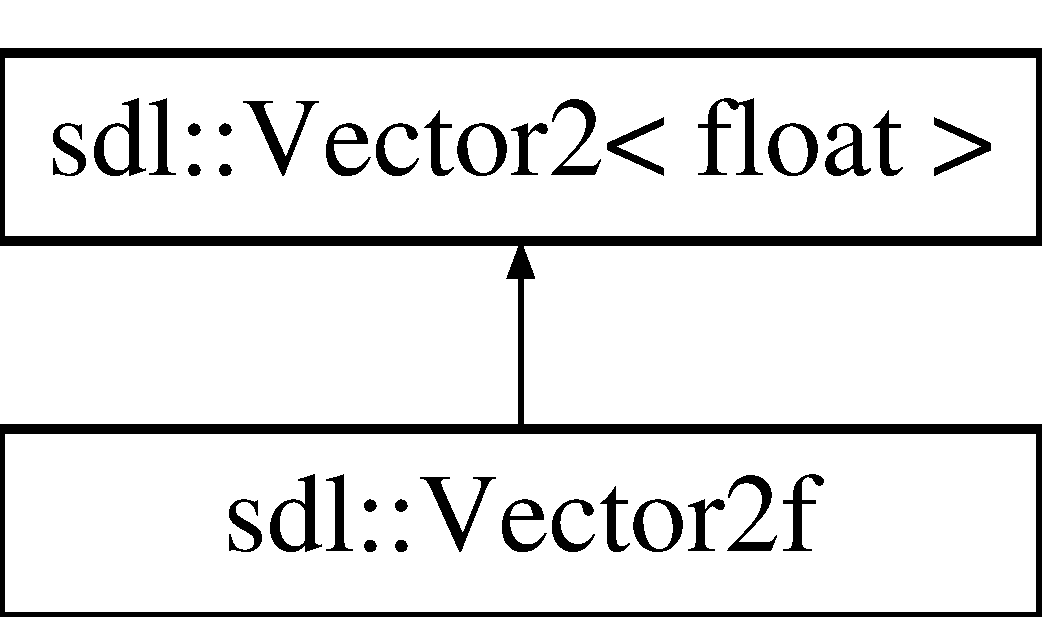
\includegraphics[height=2.000000cm]{classsdl_1_1Vector2f}
\end{center}
\end{figure}
\subsection*{Public Member Functions}
\begin{DoxyCompactItemize}
\item 
\hypertarget{classsdl_1_1Vector2f_ae789e521778c03e030d83f6076e50be9}{{\bfseries Vector2f} (const float x\-\_\-, const float y\-\_\-)}\label{classsdl_1_1Vector2f_ae789e521778c03e030d83f6076e50be9}

\item 
\hypertarget{classsdl_1_1Vector2f_a80edfede98ea588814a56c7fbb620a68}{\hyperlink{classsdl_1_1Vector2f}{Vector2f} \& {\bfseries operator/=} (const float k)}\label{classsdl_1_1Vector2f_a80edfede98ea588814a56c7fbb620a68}

\item 
\hypertarget{classsdl_1_1Vector2f_a03c6d398154d06f9f5a5c932852a0ff6}{float {\bfseries Length\-Squared} () const }\label{classsdl_1_1Vector2f_a03c6d398154d06f9f5a5c932852a0ff6}

\item 
\hypertarget{classsdl_1_1Vector2f_a768905e6443b054a5ab34678f9228502}{float {\bfseries Length} () const }\label{classsdl_1_1Vector2f_a768905e6443b054a5ab34678f9228502}

\item 
\hypertarget{classsdl_1_1Vector2f_ac3cf1bea3e4ae0a385c472e49019e992}{void {\bfseries Normalize} ()}\label{classsdl_1_1Vector2f_ac3cf1bea3e4ae0a385c472e49019e992}

\end{DoxyCompactItemize}
\subsection*{Additional Inherited Members}


The documentation for this class was generated from the following file\-:\begin{DoxyCompactItemize}
\item 
include/Vector2f.\-h\end{DoxyCompactItemize}

\hypertarget{classsdl_1_1View}{\section{sdl\-:\-:View Class Reference}
\label{classsdl_1_1View}\index{sdl\-::\-View@{sdl\-::\-View}}
}
\subsection*{Public Member Functions}
\begin{DoxyCompactItemize}
\item 
\hypertarget{classsdl_1_1View_a65409de0761dc4c3afa4098f587812a6}{{\bfseries View} (const \hyperlink{classsdl_1_1Vector2f}{Vector2f} \&pos, const \hyperlink{classsdl_1_1Vector2f}{Vector2f} \&size)}\label{classsdl_1_1View_a65409de0761dc4c3afa4098f587812a6}

\item 
\hypertarget{classsdl_1_1View_a292bdec8f5da4a4ceb78a43c6de2e482}{\hyperlink{classsdl_1_1Vector2f}{Vector2f} {\bfseries Get\-Position} () const }\label{classsdl_1_1View_a292bdec8f5da4a4ceb78a43c6de2e482}

\item 
\hypertarget{classsdl_1_1View_aa84b47ca6ca27bdea7c148be54c9dc01}{void {\bfseries Set\-Position} (const \hyperlink{classsdl_1_1Vector2f}{Vector2f} \&pos)}\label{classsdl_1_1View_aa84b47ca6ca27bdea7c148be54c9dc01}

\item 
\hypertarget{classsdl_1_1View_ab0ff71bba39b833207cd775f7c87a7b7}{void {\bfseries Move} (const \hyperlink{classsdl_1_1Vector2f}{Vector2f} \&vec)}\label{classsdl_1_1View_ab0ff71bba39b833207cd775f7c87a7b7}

\item 
\hypertarget{classsdl_1_1View_a5cb51d8ad6215d592d3c4bf78e2dc3d0}{\hyperlink{classsdl_1_1Vector2f}{Vector2f} {\bfseries Raster\-To\-World} (const \hyperlink{classsdl_1_1Vector2}{Vector2i} \&pos) const }\label{classsdl_1_1View_a5cb51d8ad6215d592d3c4bf78e2dc3d0}

\item 
\hypertarget{classsdl_1_1View_a89feab9b8b309cd4fbeddcc11623dadf}{\hyperlink{classsdl_1_1Vector2}{Vector2i} {\bfseries World\-To\-Raster} (const \hyperlink{classsdl_1_1Vector2f}{Vector2f} \&pos) const }\label{classsdl_1_1View_a89feab9b8b309cd4fbeddcc11623dadf}

\end{DoxyCompactItemize}


The documentation for this class was generated from the following files\-:\begin{DoxyCompactItemize}
\item 
include/View.\-h\item 
src/View.\-cpp\end{DoxyCompactItemize}

\hypertarget{classsdl_1_1Window}{\section{sdl\-:\-:Window Class Reference}
\label{classsdl_1_1Window}\index{sdl\-::\-Window@{sdl\-::\-Window}}
}
\subsection*{Public Member Functions}
\begin{DoxyCompactItemize}
\item 
\hypertarget{classsdl_1_1Window_a39a26091aa3fcd8b043816d33e57b91b}{{\bfseries Window} (const std\-::string name)}\label{classsdl_1_1Window_a39a26091aa3fcd8b043816d33e57b91b}

\item 
\hypertarget{classsdl_1_1Window_a8c1dcdc6090279451e96461d378722a4}{{\bfseries Window} (const std\-::string name, const int width, const int height)}\label{classsdl_1_1Window_a8c1dcdc6090279451e96461d378722a4}

\item 
\hypertarget{classsdl_1_1Window_a3368086b9e159382ebf5b1e23c905a06}{{\bfseries Window} (const std\-::string name, const uint32\-\_\-t flags)}\label{classsdl_1_1Window_a3368086b9e159382ebf5b1e23c905a06}

\item 
\hypertarget{classsdl_1_1Window_a0616c9466b4ad05efcf0a5e75cb07dc9}{{\bfseries Window} (const std\-::string name, const int width, const int height, const uint32\-\_\-t flags)}\label{classsdl_1_1Window_a0616c9466b4ad05efcf0a5e75cb07dc9}

\item 
\hypertarget{classsdl_1_1Window_a6c273a2d452fea90330fedd393eb9acb}{{\bfseries Window} (const \hyperlink{classsdl_1_1Window}{Window} \&other)=delete}\label{classsdl_1_1Window_a6c273a2d452fea90330fedd393eb9acb}

\item 
\hypertarget{classsdl_1_1Window_a871d1aa1cf1ed08cc01bb9e9c480d31a}{\hyperlink{classsdl_1_1Window}{Window} \& {\bfseries operator=} (const \hyperlink{classsdl_1_1Window}{Window} \&other)=delete}\label{classsdl_1_1Window_a871d1aa1cf1ed08cc01bb9e9c480d31a}

\item 
\hypertarget{classsdl_1_1Window_a1adff8ace96199ca503710ed191fc803}{\hyperlink{classsdl_1_1Vector2}{Vector2i} {\bfseries Get\-Size} () const }\label{classsdl_1_1Window_a1adff8ace96199ca503710ed191fc803}

\item 
\hypertarget{classsdl_1_1Window_a13592c51d1a4986454d04c68c155f3a2}{\hyperlink{classsdl_1_1Renderer}{Renderer} $\ast$ {\bfseries Create\-Renderer} ()}\label{classsdl_1_1Window_a13592c51d1a4986454d04c68c155f3a2}

\item 
\hypertarget{classsdl_1_1Window_a2cea0d565cea2658bdf53b7ee561f68a}{\hyperlink{classsdl_1_1Renderer}{Renderer} $\ast$ {\bfseries Create\-Renderer} (const uint32\-\_\-t flags)}\label{classsdl_1_1Window_a2cea0d565cea2658bdf53b7ee561f68a}

\end{DoxyCompactItemize}


The documentation for this class was generated from the following files\-:\begin{DoxyCompactItemize}
\item 
include/Window.\-h\item 
src/Window.\-cpp\end{DoxyCompactItemize}

%--- End generated contents ---

% Index
\newpage
\phantomsection
\addcontentsline{toc}{chapter}{Index}
\printindex

\end{document}
